%!TEX TS-program = pdflatexmk

% Copyright 2018 Martin Scheidt (ISC license)
% Permission to use, copy, modify, and/or distribute this file for any purpose with or without fee is hereby granted, provided that the above copyright notice and this permission notice appear in all copies.

\documentclass[tikz,border=2]{standalone}

\usepackage{lmodern}
\usepackage[prefix=]{xcolor-solarized}

\def\rootTrackschematic{../../tikz-trackschematic}
\def\srcTrackschematic{\rootTrackschematic/src}
%% symbol library for TikZ track schematics
%
% Copyright 2019 Martin Scheidt (ISC license)

% Permission to use, copy, modify, and/or distribute this file for any purpose with or without fee is hereby granted, provided that the above copyright notice and this permission notice appear in all copies.

\colorlet{background}{white}
\colorlet{foreground}{black}

\tikzset{MainTrack/.style={line width=2pt,foreground}}
\tikzset{SideTrack/.style={line width=0.7pt,foreground}}

\tikzset{
  pics/track_number/.style args={#1}{
    code={
      \node[fill=background,font=\sffamily,text=foreground] at (0,0) {#1}; % speed indicator
    }
  },
  pics/track_number/.default=,
}
\tikzset{
  pics/track_distance/.style args={#1}{
    code={
      \fill[foreground] (0,0.96) -- ++(-0.1,-0.15) -- ++(0.2,0) -- cycle; % upper triangle
      \node[baseline=(current bounding box.center),font=\sffamily,text=foreground] at (0,0.5) {#1}; % distance indicator
      \fill[foreground] (0,0.04) -- ++(-0.1,0.15) -- ++(0.2,0) -- cycle; % lower triangle
    }
  },
  pics/track_distance/.default=,
}
\tikzset{
  pics/turnout_left_forward/.style args={#1}{
    code={
      \path[draw=foreground,line width=1pt,fill=#1] (0,0) --  ++(0.4,0.4) -- ++(0,-0.4); % turnout marker
    }
  },
  pics/turnout_left_forward/.default=foreground,
}
\tikzset{
  pics/turnout_left_backward/.style args={#1}{
    code={
      \path[draw=foreground,line width=1pt,fill=#1] (0,0) --  ++(-0.4,-0.4) -- ++(0,0.4); % turnout marker
    }
  },
  pics/turnout_left_backward/.default=foreground,
}
\tikzset{
  pics/turnout_right_forward/.style args={#1}{
    code={
      \path[draw=foreground,line width=1pt,fill=#1] (0,0) --  ++(0.4,-0.4) -- ++(0,0.4); % turnout marker
    }
  },
  pics/turnout_right_forward/.default=foreground,
}
\tikzset{
  pics/turnout_right_backward/.style args={#1}{
    code={
      \path[draw=foreground,line width=1pt,fill=#1] (0,0) --  ++(-0.4,0.4) -- ++(0,-0.4); % turnout marker
    }
  },
  pics/turnout_right_backward/.default=foreground,
}
\tikzset{
  fouling_point_right_backward/.pic={
    \path[draw=foreground,line width=0.75pt] (-0.7,0) --  ++(0,0.7); % fouling point indicator
  };
}
\tikzset{
  fouling_point_left_backward/.pic={
    \path[draw=foreground,line width=0.75pt] (-0.7,0) --  ++(0,-0.7); % fouling point indicator
  };
}
\tikzset{
  fouling_point_right_forward/.pic={
    \path[draw=foreground,line width=0.75pt] (0.7,0) --  ++(0,-0.7); % fouling point indicator
  };
}
\tikzset{
  fouling_point_left_forward/.pic={
    \path[draw=foreground,line width=0.75pt] (0.7,0) --  ++(0,0.7); % fouling point indicator
  };
}
\tikzset{
  slip_left_forward/.pic={
    \path[draw=foreground,line width=0.75pt] (-0.4,0.1) --  (0.3,0.4); % fouling point indicator
  };
}
\tikzset{
  slip_left_backward/.pic={
    \path[draw=foreground,line width=0.75pt] (-0.3,-0.4) --  (0.4,-0.1); % fouling point indicator
  };
}
\tikzset{
  slip_right_forward/.pic={
    \path[draw=foreground,line width=0.75pt] (-0.4,-0.1) --  (0.3,-0.4); % fouling point indicator
  };
}
\tikzset{
  slip_right_backward/.pic={
    \path[draw=foreground,line width=0.75pt] (0.4,0.1) --  (-0.3,0.4); % fouling point indicator
  };
}
\tikzset{
  turnout_left_forward_points_right/.pic={
    \path[draw=foreground,line width=1.5pt] (0,-0.1) -- ++(0.3,0); % points indicator
  };
}
\tikzset{
  turnout_left_forward_points_left/.pic={
    \path[draw=foreground,line width=1.5pt] (-0.035, 0.1) -- ++(0.2,0.2); % points indicator
  };
}
\tikzset{
  turnout_left_forward_points_moving/.pic={
    \fill[foreground] (0.075,-0.1) circle (0.05); % points indicator left
    \fill[foreground] (0.225,-0.1) circle (0.05);
    \fill[foreground] (0.015, 0.15) circle (0.05); % points indicator right
    \fill[foreground] (0.115, 0.25) circle (0.05);
  };
}
\tikzset{
  turnout_left_backward_points_right/.pic={
    \path[draw=foreground,line width=1.5pt] (0,0.1) -- ++(-0.3,0); % points indicator
  };
}
\tikzset{
  turnout_left_backward_points_left/.pic={
    \path[draw=foreground,line width=1.5pt] (0.035,-0.1) -- ++(-0.2,-0.2); % points indicator
  };
}
\tikzset{
  turnout_left_backward_points_moving/.pic={
    \fill[foreground] (-0.075,0.1) circle (0.05); % points indicator left
    \fill[foreground] (-0.225,0.1) circle (0.05);
    \fill[foreground] (-0.015,-0.15) circle (0.05); % points indicator right
    \fill[foreground] (-0.115,-0.25) circle (0.05);
  };
}
\tikzset{
  turnout_right_forward_points_right/.pic={
    \path[draw=foreground,line width=1.5pt] (-0.035,-0.1) -- ++(0.2,-0.2); % points indicator
  };
}
\tikzset{
  turnout_right_forward_points_left/.pic={
    \path[draw=foreground,line width=1.5pt] (0,0.1) -- ++(0.3,0); % points indicator
  };
}
\tikzset{
  turnout_right_forward_points_moving/.pic={
    \fill[foreground] (0.075, 0.1) circle (0.05); % points indicator left
    \fill[foreground] (0.225, 0.1) circle (0.05);
    \fill[foreground] (0.015,-0.15) circle (0.05); % points indicator right
    \fill[foreground] (0.115,-0.25) circle (0.05);
  };
}
\tikzset{
  turnout_right_backward_points_right/.pic={
    \path[draw=foreground,line width=1.5pt] (0.035,0.1) -- ++(-0.2,0.2); % points indicator
  };
}
\tikzset{
  turnout_right_backward_points_left/.pic={
    \path[draw=foreground,line width=1.5pt] (0,-0.1) -- ++(-0.3,0); % points indicator
  };
}
\tikzset{
  turnout_right_backward_points_moving/.pic={
    \fill[foreground] (-0.075,-0.1) circle (0.05); % points indicator left
    \fill[foreground] (-0.225,-0.1) circle (0.05);
    \fill[foreground] (-0.015,0.15) circle (0.05); % points indicator right
    \fill[foreground] (-0.115,0.25) circle (0.05);
  };
}
\tikzset{
  derailer_right_forward/.pic={
    \path[draw=foreground, line width=1pt] (0,0.2) -- ++(0,-0.4); % derailer marker
    \path[draw=foreground,->,>=latex,line width=1pt,dashed] (0,0) -- ++(0.4,-0.4); % derailer arrow
  };
}
\tikzset{
  derailer_right_backward/.pic={
    \path[draw=foreground, line width=1pt] (0,0.2) -- ++(0,-0.4); % derailer marker
    \path[draw=foreground,->,>=latex,line width=1pt,dashed] (0,0) -- ++(-0.4,0.4); % derailer arrow
  };
}
\tikzset{
  derailer_left_forward/.pic={
    \path[draw=foreground, line width=1pt] (0,0.2) -- ++(0,-0.4); % derailer marker
    \path[draw=foreground,->,>=latex,line width=1pt,dashed] (0,0) -- ++(0.4,0.4); % derailer arrow
  };
}
\tikzset{
  derailer_left_backward/.pic={
    \path[draw=foreground, line width=1pt] (0,0.2) -- ++(0,-0.4); % derailer marker
    \path[draw=foreground,->,>=latex,line width=1pt,dashed] (0,0) -- ++(-0.4,-0.4); % derailer arrow
  };
}
\tikzset{
  bufferstop_forward/.pic={
    \path[draw=foreground, line width=1pt] (-0.1,0.2) --  ++(0.1,0) -- ++(0,-0.4) -- ++ (-0.1,0); % bufferstop marker
  };
}
\tikzset{
  bufferstop_backward/.pic={
    \path[draw=foreground, line width=1pt] (0.1,0.2) --  ++(-0.1,0) -- ++(0,-0.4) -- ++ (0.1,0); % bufferstop marker
  };
}

%% symbol library for TikZ track schematics
%
% Copyright 2018 Martin Scheidt (ISC license)

% Permission to use, copy, modify, and/or distribute this file for any purpose with or without fee is hereby granted, provided that the above copyright notice and this permission notice appear in all copies.

\tikzset{
  train_berth_sign_forward/.pic={
    \path[draw, line width=1pt] (0,0) -- ++(0,-0.4) -- ++(0.3,0); % signal pole
    {   % signal marker
      \path[draw, line width=1pt] (0.3,-0.575) rectangle ++(0.5,0.35);
      \path[draw, line width=0.75pt] (0.375,-0.3) -- ++(0.35,0);
      \path[draw, line width=0.75pt] (0.55,-0.5) -- ++(0,0.2);
      \path[draw, line width=0.75pt] (0.375,-0.5) -- ++(0.35,0);
    }
  };
}
\tikzset{
  train_berth_sign_backward/.pic={
    \path[draw, line width=1pt] (0,0) -- ++(0,0.4) -- ++(-0.3,0); % signal pole
    {   % signal marker
      \path[draw, line width=1pt] (-0.3,0.575) rectangle ++(-0.5,-0.35);
      \path[draw, line width=0.75pt] (-0.375,0.3) -- ++(-0.35,0);
      \path[draw, line width=0.75pt] (-0.55,0.5) -- ++(0,-0.2);
      \path[draw, line width=0.75pt] (-0.375,0.5) -- ++(-0.35,0);
    }
  };
}
\tikzset{
  pics/train_berth_shape/.style n args={1}{
    code={
      \path[draw,line width=0.75pt,densely dotted] (0, 0.25) -- (0, 0.35) -- (#1, 0.35) -- ++(0,-0.1); % berth shape
      \path[draw,line width=0.75pt,densely dotted] (0,-0.25) -- (0,-0.35) -- (#1,-0.35) -- ++(0, 0.1); % berth shape
    }
  },
  pics/train_berth_shape/.default=4,
}
\tikzset{
  pics/train_berth_shape_forward/.style n args={1}{
    code={
      \path[draw,line width=0.75pt,densely dotted] (0,-0.25) -- (0,-0.35) -- (#1,-0.35) -- ++(0, 0.1); % berth shape
    }
  },
  pics/train_berth_shape/.default=4,
}
\tikzset{
  pics/train_berth_shape_backward/.style n args={1}{
    code={
      \path[draw,line width=0.75pt,densely dotted] (0, 0.25) -- (0, 0.35) -- (#1, 0.35) -- ++(0,-0.1); % berth shape
    }
  },
  pics/train_berth_shape/.default=4,
}
\tikzset{
  view_point_forward/.pic={
    \path[draw,<-,>=latex,line width=1pt] (0,-0.1) -- ++(0,-0.3) -- ++(0.2,0); % arrow
    { % eye
    \filldraw (0.4,-0.4) circle (0.1);
    \path[draw, line width=1pt]
      (0.4,-0.15) .. controls (0.25,-0.25) and (0.25,-0.55) .. (0.4,-0.65) .. controls (0.55,-0.55) and (0.55,-0.25) .. (0.4,-0.15)--cycle;
    }
  };
}
\tikzset{
  view_point_backward/.pic={
    \tikzset{>=latex}
    \path[draw,<-,>=latex,line width=1pt] (0,0.1) -- ++(0,0.3) -- ++(-0.2,0); % arrow
    { % eye
    \filldraw (-0.4,0.4) circle (0.1);
    \path[draw, line width=1pt]
      (-0.4,0.15) .. controls (-0.25,0.25) and (-0.25,0.55) .. (-0.4,0.65) .. controls (-0.55,0.55) and (-0.55,0.25) .. (-0.4,0.15)--cycle;
    }
  };
}
\tikzset{
  pics/distant_signal_forward/.style args={#1}{
    code={
      \path[draw, line width=1pt] (0,0) -- ++(0,-0.4) -- ++(0.4,0); % signal pole
      \path[draw, line width=1pt] (0.7,-0.6) -- ++(0,0.4) -- ++ (-0.35,-0.2) -- cycle; % signal marker
      \node[rotate=-90,font=\sffamily] at (0.9,-0.4) {#1}; % speed indicator
    }
  },
  pics/distant_signal_forward/.default=,
}
\tikzset{
  pics/distant_signal_backward/.style args={#1}{
    code={
      \path[draw, line width=1pt] (0,0) -- ++(0,0.4) -- ++(-0.4,0); % signal pole
      \path[draw, line width=1pt] (-0.7,0.6) -- ++(0,-0.4) -- ++ (0.35,0.2) -- cycle; % signal marker
      \node[rotate=90,font=\sffamily] at (-0.9,0.4) {#1}; % speed indicator
    }
  },
  pics/distant_signal_backward/.default=,
}
\tikzset{
  pics/speed_signal_forward/.style args={#1}{
    code={
      \path[draw, line width=1pt] (0,0) -- ++(0,-0.4) -- ++(0.4,0); % signal pole
      \path[draw, line width=1pt] (0.4,-0.2) -- ++(0,-0.4) -- ++ (0.35,0.2) -- cycle; % signal marker
      \node[rotate=-90,font=\sffamily] at (0.9,-0.4) {#1}; % speed indicator
    }
  },
  pics/speed_signal_forward/.default=,
}
\tikzset{
  pics/speed_signal_backward/.style args={#1}{
    code={
      \path[draw, line width=1pt] (0,0) -- ++(0,0.4) -- ++(-0.4,0); % signal pole
      \path[draw, line width=1pt] (-0.4,0.2) -- ++(0,0.4) -- ++ (-0.35,-0.2) -- cycle; % signal marker
      \node[rotate=90,font=\sffamily] at (-0.9,0.4) {#1}; % speed indicator
    }
  },
  pics/speed_signal_backward/.default=,
}
\tikzset{
  pics/block_signal_forward/.style args={#1}{
    code={
      \path[draw, line width=1pt] (0,0) -- ++(0,-0.4) -- ++(0.7,0); % signal pole
      \path[draw, line width=1pt] (0.7,-0.6) rectangle ++(0.4,0.4); % signal marker
      \node[rotate=-90,font=\sffamily] at (1.2,-0.4) {#1}; % speed indicator
    }
  },
  pics/block_signal_forward/.default=,
}
\tikzset{
  pics/block_signal_backward/.style args={#1}{
    code={
      \path[draw, line width=1pt] (0,0) -- ++(0,0.4) -- ++(-0.7,0); % signal pole
      \path[draw, line width=1pt] (-0.7,0.6) rectangle ++(-0.4,-0.4); % signal marker
      \node[rotate=90,font=\sffamily] at (-1.2,0.4) {#1}; % speed indicator
    }
  },
  pics/block_signal_backward/.default=,
}
\tikzset{
  pics/route_signal_forward/.style args={#1}{
    code={
      \path[draw, line width=1pt] (0,0) -- ++(0,-0.4) -- ++(0.7,0); % signal pole
      \path[draw, line width=1pt] (0.9,-0.4) circle (0.2); % signal marker
      \node[rotate=-90,font=\sffamily] at (1.2,-0.4) {#1}; % speed indicator
    }
  },
  pics/route_signal_forward/.default=,
}
\tikzset{
  pics/route_signal_backward/.style args={#1}{
    code={
      \path[draw, line width=1pt] (0,0) -- ++(0,0.4) -- ++(-0.7,0); % signal pole
      \path[draw, line width=1pt] (-0.9,0.4) circle (0.2); % signal marker
      \node[rotate=90,font=\sffamily] at (-1.2,0.4) {#1}; % speed indicator
    }
  },
  pics/route_signal_backward/.default=,
}
\tikzset{
  shunt_signal_forward/.pic={
    \path[draw, line width=1pt] (0,0) -- ++(0,-0.4) -- ++(0.7,0); % signal pole
    \path[draw, line width=1pt] (0.6,-0.3) circle (0.1); % signal marker
  };
}
\tikzset{
  shunt_signal_backward/.pic={
    \path[draw, line width=1pt] (0,0) -- ++(0,0.4) -- ++(-0.7,0); % signal pole
    \path[draw, line width=1pt] (-0.6,0.3) circle (0.1); % signal marker
  };
}
\tikzset{
  shunt_limit_forward/.pic={
    \path[draw, line width=1pt] (0,0) -- ++(0,-0.4) -- ++(0.5,0); % signal pole
    \path[draw, line width=1pt] (0.5,-0.25) arc (270:90:-0.15) -- cycle;; % signal marker
  };
}
\tikzset{
  shunt_limit_backward/.pic={
    \path[draw, line width=1pt] (0,0) -- ++(0,0.4) -- ++(-0.5,0); % signal pole
    \path[draw, line width=1pt] (-0.5,0.55) arc (90:270:0.15) -- cycle;; % signal marker
  };
}
\tikzset{
  block_end_marker_forward/.pic={
    \path[draw, line width=1pt] (0,0) -- ++(0,-0.5); % marker
    \path[draw, line width=1pt] (-0.1,-0.7) rectangle ++(0.2,0.2); % sign
  };
}
\tikzset{
  block_end_marker_backward/.pic={
    \path[draw, line width=1pt] (0,0) -- ++(0,0.5); % marker
    \path[draw, line width=1pt] (0.1,0.7) rectangle ++(-0.2,-0.2); % sign
  };
}
\tikzset{
  block_clearing_point_forward/.pic={
    \path[draw, line width=1pt] (0,0.1) -- ++(0,-0.2); % marker
    \path[draw, line width=1pt] (0,-0.1) -- ++(-0.1,-0.1) -- ++(0.1,-0.1) -- ++(0.1,0.1) -- cycle; % sign
  };
}
\tikzset{
  block_clearing_point_backward/.pic={
    \path[draw, line width=1pt] (0,-0.1) -- ++(0,0.2); % marker
    \path[draw, line width=1pt] (0,0.1) -- ++(0.1,0.1) -- ++(-0.1,0.1) -- ++(-0.1,-0.1) -- cycle; % sign
  };
}
\tikzset{
  route_clearing_point_forward/.pic={
    \path[draw, line width=1pt] (0,0.1) -- ++(0,-0.2); % marker
    \path[draw, line width=1pt] (0,-0.2) circle (0.1); % sign
  };
}
\tikzset{
  route_clearing_point_backward/.pic={
    \path[draw, line width=1pt] (0,-0.1) -- ++(0,0.2); % marker
    \path[draw, line width=1pt] (0, 0.2) circle (0.1); % sign
  };
}
\tikzset{
  clearing_point/.pic={
    \path[draw, line width=1pt] (0  ,-0.1) -- ++( 0  ,0.2); % marker
    \path[draw, line width=1pt] (0.1, 0.1) -- ++(-0.2,0  ); % sign
  };
}
\tikzset{
  pics/transmitter_below/.style args={#1}{
    code={
      \path[draw,line width=1pt,fill=#1] (-0.25,0) rectangle (0.25,-0.25); % turnout marker
    }
  },
  pics/transmitter_below/.default=white,
}
\tikzset{
  pics/transmitter_below_forward/.style args={#1}{
    code={
      \path[draw,line width=1pt,fill=#1] (-0.25,0) rectangle (0.25,-0.25); % turnout marker
      \path[draw] (0.1,-0.05) -- (0.2,-0.125) -- (0.1,-0.2) -- cycle;
    }
  },
  pics/transmitter_below_forward/.default=white,
}
\tikzset{
  pics/transmitter_below_backward/.style args={#1}{
    code={
      \path[draw,line width=1pt,fill=#1] (-0.25,0) rectangle (0.25,-0.25); % turnout marker
      \path[draw] (-0.1,-0.05) -- (-0.2,-0.125) -- (-0.1,-0.2) -- cycle;
    }
  },
  pics/transmitter_below_backward/.default=white,
}
\tikzset{
  pics/transmitter_below_bidirectional/.style args={#1}{
    code={
      \path[draw,line width=1pt,fill=#1] (-0.25,0) rectangle (0.25,-0.25); % turnout marker
      \path[draw] ( 0.1,-0.05) -- ( 0.2,-0.125) -- ( 0.1,-0.2) -- cycle;
      \path[draw] (-0.1,-0.05) -- (-0.2,-0.125) -- (-0.1,-0.2) -- cycle;
    }
  },
  pics/transmitter_below_bidirectional/.default=white,
}
\tikzset{
  pics/transmitter_above/.style args={#1}{
    code={
      \path[draw,line width=1pt,fill=#1] (-0.25,0) rectangle (0.25,0.25); % turnout marker
    }
  },
  pics/transmitter_above/.default=white,
}
\tikzset{
  pics/transmitter_above_forward/.style args={#1}{
    code={
      \path[draw,line width=1pt,fill=#1] (-0.25,0) rectangle (0.25,0.25); % turnout marker
      \path[draw] (0.1,0.05) -- (0.2,0.125) -- (0.1,0.2) -- cycle;
    }
  },
  pics/transmitter_above_forward/.default=white,
}
\tikzset{
  pics/transmitter_above_backward/.style args={#1}{
    code={
      \path[draw,line width=1pt,fill=#1] (-0.25,0) rectangle (0.25,0.25); % turnout marker
      \path[draw] (-0.1,0.05) -- (-0.2,0.125) -- (-0.1,0.2) -- cycle;
    }
  },
  pics/transmitter_above_backward/.default=white,
}
\tikzset{
  pics/transmitter_above_bidirectional/.style args={#1}{
    code={
      \path[draw,line width=1pt,fill=#1] (-0.25,0) rectangle (0.25,0.25); % turnout marker
      \path[draw] ( 0.1,0.05) -- ( 0.2,0.125) -- ( 0.1,0.2) -- cycle;
      \path[draw] (-0.1,0.05) -- (-0.2,0.125) -- (-0.1,0.2) -- cycle;
    }
  },
  pics/transmitter_above_bidirectional/.default=white,
}
%% symbol library for TikZ track schematics
%
% Copyright 2018 Martin Scheidt (ISC license)

% Permission to use, copy, modify, and/or distribute this file for any purpose with or without fee is hereby granted, provided that the above copyright notice and this permission notice appear in all copies.

\tikzset{
  pics/platform_left/.style n args={1}{
    code={
      \path[draw, line width=0.75pt] (0,0.5) -- ++(0,-0.3) -- ++(#1,0) -- ++(0,0.3);
      \path[draw, line width=0.75pt] (0,0.3) -- ++(#1,0);
    }
  },
  pics/platform_left/.default=4,
}
\tikzset{
  pics/platform_right/.style n args={1}{
    code={
      \path[draw, line width=0.75pt] (0,-0.5) -- ++(0,0.3) -- ++(#1,0) -- ++(0,-0.3);
      \path[draw, line width=0.75pt] (0,-0.3) -- ++(#1,0);
    }
  },
  pics/platform_right/.default=4,
}
\tikzset{
  level_crossing_barrier_left/.pic={
    { % road
      \path[draw, line width=1pt] (-0.2, 0.8) --  ++(0,-0.6);
      \path[draw, line width=1pt] ( 0.2, 0.8) --  ++(0,-0.6);
    }
    { % barrier
      \filldraw (-0.4,0.5) circle (0.05);
      \path[draw, line width=1pt] (-0.4,0.5) --  ++(0.39,0);
    }
  };
}
\tikzset{
  level_crossing_barrier_right/.pic={
    { % road
      \path[draw, line width=1pt] (-0.2,-0.8) --  ++(0, 0.6);
      \path[draw, line width=1pt] ( 0.2,-0.8) --  ++(0, 0.6);
    }
    { % barrier
      \filldraw (0.4,-0.5) circle (0.05);
      \path[draw, line width=1pt] (0.4,-0.5) --  ++(-0.39,0);
    }
  };
}
\tikzset{
  level_crossing/.pic={
    { % road
      \path[draw, line width=1pt] (-0.2,-0.8) --  ++(0, 0.6);
      \path[draw, line width=1pt] ( 0.2,-0.8) --  ++(0, 0.6);
    }
  };
}
\tikzset{
  pics/bridge_left/.style n args={1}{
    code={
      \path[draw, line width=0.75pt] (-0.1,0.48) --  ++(0.08,-0.08) -- ++(#1,0) -- ++(0.08,0.08);
    }
  },
  pics/bridge_left/.default=3,
}
\tikzset{
  pics/bridge_right/.style n args={1}{
    code={
      \path[draw, line width=0.75pt] (-0.1,-0.48) --  ++(0.08,0.08) -- ++(#1,0) -- ++(0.08,-0.08);
    }
  },
  pics/bridge_right/.default=3,
}


\begin{document}
  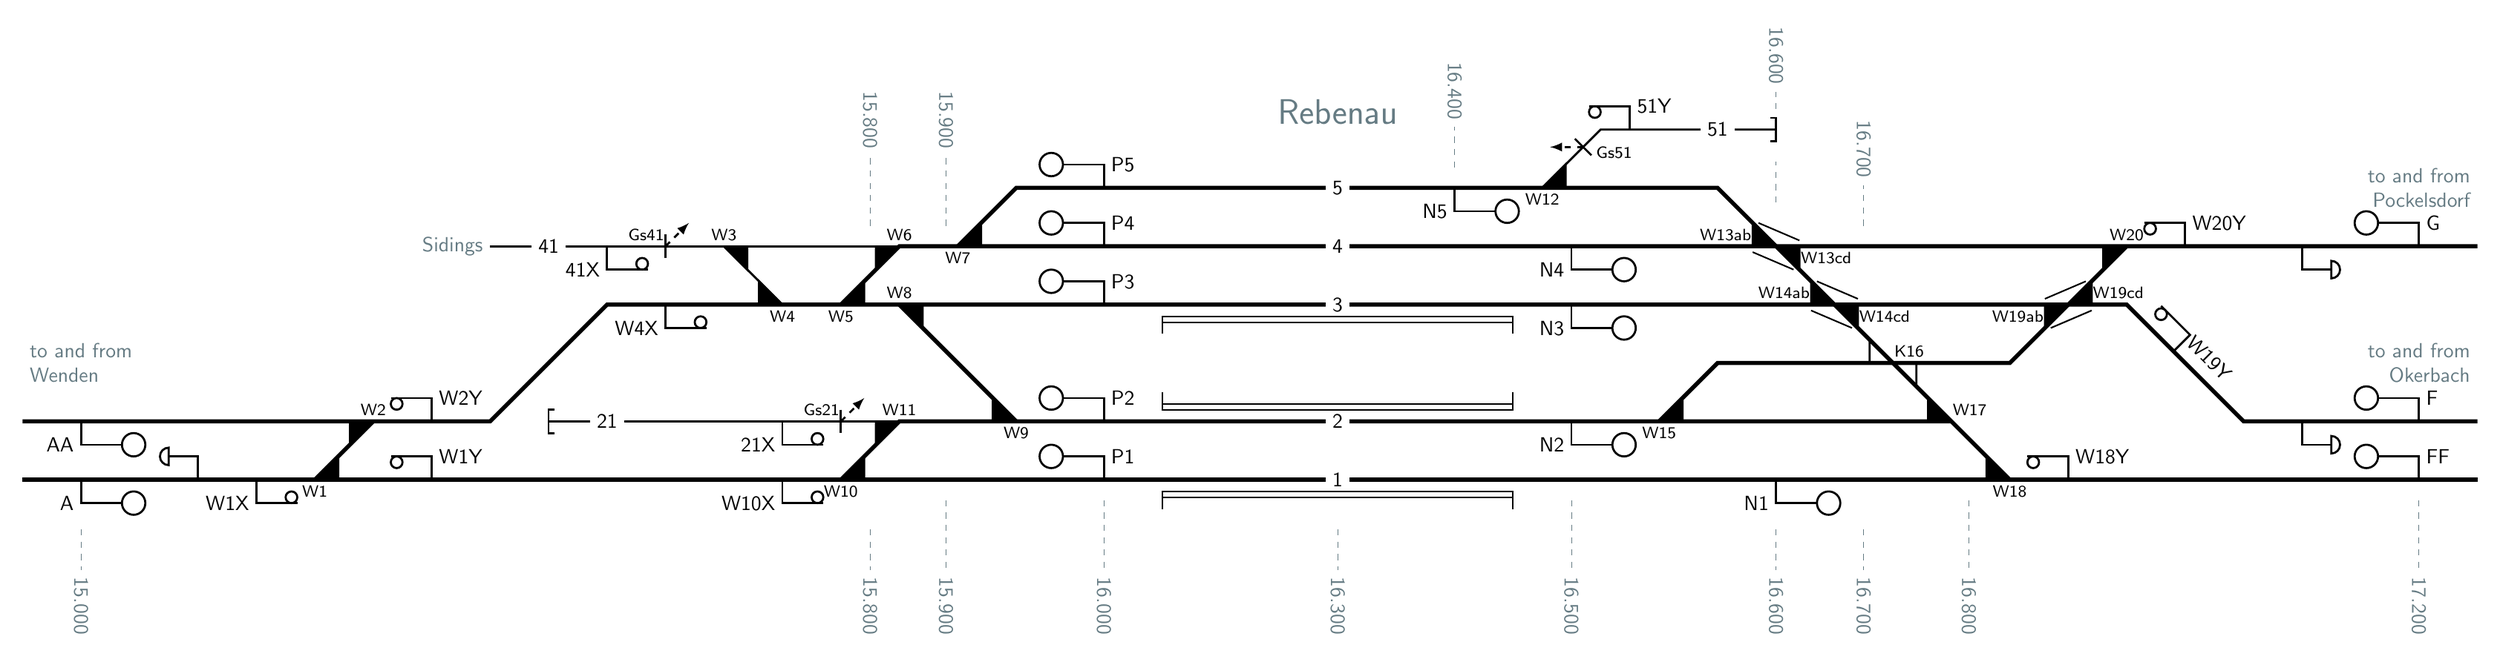
\begin{tikzpicture}[font=\sffamily]
  {   % stations
    \tikzset{every node/.style={base00}};
    \node[right,align=left] at ( 0,2) {to and from\\ Wenden};
    \node[left,align=right] at ( 8,4.0) {Sidings};
    \node                   at (22.5,6.3) {{\LARGE Rebenau}};
    \node[left,align=right] at (42,2) {to and from\\ Okerbach};
    \node[left,align=right] at (42,5) {to and from\\ Pockelsdorf};
  }
  {   % tracks
    \draw[line width=2pt] ( 0, 0) -- ++(42, 0); % track 1
    \draw[line width=2pt] ( 5, 0) -- ++( 1, 1);
    \draw[line width=2pt] ( 0, 1) -- ++( 8, 0) -- ++(2,2) -- ++(26,0) -- ++(2,-2) -- ++(4,0);  % track 3
    \draw[line width=1pt] ( 9, 1) -- ++( 6, 0); % track 21
    \draw[line width=1pt] ( 8, 4) -- ++( 7, 0); % track 41
    \draw[line width=1pt] (12, 4) -- ++( 1,-1);
    \draw[line width=2pt] (14, 3) --   (15, 4) -- ++(27,0);  % track 4
    \draw[line width=2pt] (14, 0) -- ++( 1, 1) -- ++(18, 0); % track 2
    \draw[line width=2pt] (15, 3) -- ++( 2,-2);
    \draw[line width=2pt] (16, 4) --   (17, 5) -- (29, 5) -- ++(5,-5); % track 5
    \draw[line width=2pt] (28, 1) -- ++( 1, 1) -- ++(5,0) -- ++ (2,2);
    \draw[line width=1pt] (26, 5) -- ++( 1, 1) -- ++(3,0);  % track 51

    % track numbers
    \node[fill=white] at ( 9.0, 4) {41};
    \node[fill=white] at (10.0, 1) {21};
    \node[fill=white] at (22.5, 0) { 1};
    \node[fill=white] at (22.5, 1) { 2};
    \node[fill=white] at (22.5, 3) { 3};
    \node[fill=white] at (22.5, 4) { 4};
    \node[fill=white] at (22.5, 5) { 5};
    \node[fill=white] at (29.0, 6) {51};
    % % bufferstops
    \pic  at ( 9, 1) {bufferstop_backward};
    \pic  at (30, 6) {bufferstop_forward};
    % turnouts
    \pic  at ( 5,0) {turnout_left_forward};
    \node at ( 5,-0.2) {\footnotesize W1};
    % \pic at ( 5,0) {fouling_point_left_forward};
    \pic  at ( 6,1) {turnout_left_backward};
    \node at ( 6,1.2) {\footnotesize W2};
    % \pic at ( 6,1) {fouling_point_left_backward};
    \pic  at (11,4) {derailer_left_forward};
    \node[left,align=right] at (11.1,4.2) {\footnotesize Gs41};
    \pic  at (12,4) {turnout_right_forward};
    \node at (12,4.2) {\footnotesize W3};
    % \pic at (12,4) {fouling_point_right_forward};
    \pic  at (13,3) {turnout_right_backward};
    \node at (13,2.8) {\footnotesize W4};
    % \pic at (13,3) {fouling_point_right_backward};
    \pic  at (14,3) {turnout_left_forward};
    \node at (14,2.8) {\footnotesize W5};
    % \pic at (14,3) {fouling_point_left_forward};
    \pic  at (15,4) {turnout_left_backward};
    \node at (15,4.2) {\footnotesize W6};
    % \pic at (15,4) {fouling_point_left_backward};
    \pic  at (14,0) {turnout_left_forward};
    \node at (14,-0.2) {\footnotesize W10};
    % \pic at (14.0,0) {fouling_point_left_forward};
    \pic  at (15,1) {turnout_left_backward};
    \node at (15,1.2) {\footnotesize W11};
    % \pic at (15,1) {fouling_point_left_backward};
    \pic  at (14,1) {derailer_left_forward};
    \node[left,align=right] at (14.1,1.2) {\footnotesize Gs21};
    \pic  at (15,3) {turnout_right_forward};
    \node at (15,3.2) {\footnotesize W8};
    % \pic at (15,3) {fouling_point_right_forward};
    \pic  at (16,4) {turnout_left_forward};
    \node at (16,3.8) {\footnotesize W7};
    % \pic at (16,4) {fouling_point_left_forward};
    \pic  at (17,1) {turnout_right_backward};
    \node at (17,0.8) {\footnotesize W9};
    % \pic at (17,1) {fouling_point_right_backward};

    \pic  at (28,1) {turnout_left_forward};
    \node at (28,0.8) {\footnotesize W15};
    % \pic at (28,1) {fouling_point_left_forward};
    \pic  at (26,5) {turnout_left_forward};
    \node at (26,4.8) {\footnotesize W12};
    % \pic at (28,5) {fouling_point_right_forward};
    \pic [rotate=45] at (26.7,5.7) {derailer_right_backward};
    \node[right,align=left] at (26.8,5.6) {\footnotesize Gs51};
    \pic  at (30,4) {turnout_right_forward};
    \pic  at (30,4) {turnout_right_backward};
    \pic  at (30,4) {slip_right_forward};
    \pic  at (30,4) {slip_right_backward};
    \node[left,align=right] at (29.7,4.2) {\footnotesize W13ab};
    \node[right,align=left] at (30.3,3.8) {\footnotesize W13cd};
    % \pic at (30,4) {fouling_point_right_backward};
    % \pic at (30,4) {fouling_point_right_forward};
    \pic  at (31,3) {turnout_right_forward};
    \pic  at (31,3) {turnout_right_backward};
    \pic  at (31,3) {slip_right_forward};
    \pic  at (31,3) {slip_right_backward};
    \node[left,align=right] at (30.7,3.2) {\footnotesize W14ab};
    \node[right,align=left] at (31.3,2.8) {\footnotesize W14cd};
    % \pic at (31,3) {fouling_point_right_backward};
    % \pic at (31,3) {fouling_point_right_forward};
    \pic  at (32,2) {turnout_right_forward=none};
    \pic  at (32,2) {turnout_right_backward=none};
    \node[right,align=left] at (31.9,2.2) {\footnotesize K16};
    % \pic at (32,2) {fouling_point_right_backward};
    % \pic at (32,2) {fouling_point_right_forward};
    \pic  at (33,1) {turnout_right_backward};
    \node[right,align=left] at (32.9,1.2) {\footnotesize W17};
    % \pic at (33,1) {fouling_point_right_backward};
    \pic  at (34,0) {turnout_right_backward};
    \node at (34,-0.2) {\footnotesize W18};
    % \pic at (34,0) {fouling_point_right_backward};
    \pic  at (35,3) {turnout_left_forward};
    \pic  at (35,3) {turnout_left_backward};
    \pic  at (35,3) {slip_left_forward};
    \pic  at (35,3) {slip_left_backward};
    \node[left,align=right] at (34.7,2.8) {\footnotesize W19ab};
    \node[right,align=left] at (35.3,3.2) {\footnotesize W19cd};
    % \pic at (35,3) {fouling_point_left_backward};
    % \pic at (35,3) {fouling_point_left_forward};
    \pic  at (36,4) {turnout_left_backward};
    \node at (36,4.2) {\footnotesize W20};
    % \pic at (36,4) {fouling_point_left_backward};

    % % platforms
    \pic  at (19.5,0) {platform_right=6};
    \pic  at (19.5,1) {platform_left=6};
    \pic  at (19.5,3) {platform_right=6};
  }
  {   % signals
    \pic at ( 1,0) {route_signal_forward};
    \node[left] at (1,-0.4) {A};
    \pic at ( 1,1) {route_signal_forward};
    \node[left] at (1, 0.6) {AA};
    \pic at ( 3,0) {shunt_limit_backward};
    \pic at ( 4,0) {shunt_signal_forward};
    \node[left] at ( 4,-0.4) {W1X};
    \pic at ( 7,1) {shunt_signal_backward};
    \node[right] at ( 7, 1.4) {W2Y};
    \pic at ( 7,0) {shunt_signal_backward};
    \node[right] at ( 7, 0.4) {W1Y};
    \pic at (11,3) {shunt_signal_forward};
    \node[left] at (11, 2.6) {W4X};
    \pic at (10,4) {shunt_signal_forward};
    \node[left] at (10, 3.6) {41X};
    \pic at (13,0) {shunt_signal_forward};
    \node[left] at (13,-0.4) {W10X};
    \pic at (13,1) {shunt_signal_forward};
    \node[left] at (13, 0.6) {21X};
    \pic at (18.5,0) {route_signal_backward};
    \node[right] at (18.5, 0.4) {P1};
    \pic at (18.5,1) {route_signal_backward};
    \node[right] at (18.5, 1.4) {P2};
    \pic at (18.5,3) {route_signal_backward};
    \node[right] at (18.5, 3.4) {P3};
    \pic at (18.5,4) {route_signal_backward};
    \node[right] at (18.5, 4.4) {P4};
    \pic at (18.5,5) {route_signal_backward};
    \node[right] at (18.5, 5.4) {P5};

    \pic at (24.5,5) {route_signal_forward};
    \node[left] at (24.5, 4.6) {N5};
    \pic at (26.5,1) {route_signal_forward};
    \node[left] at (26.5, 0.6) {N2};
    \pic at (26.5,3) {route_signal_forward};
    \node[left] at (26.5, 2.6) {N3};
    \pic at (26.5,4) {route_signal_forward};
    \node[left] at (26.5, 3.6) {N4};
    \pic at (27.5,6) {shunt_signal_backward};
    \node[right] at ( 27.5, 6.4) {51Y};
    \pic at (30.0,0) {route_signal_forward};
    \node[left] at (30.0,-0.4) {N1};
    \pic at (35.0,0) {shunt_signal_backward};
    \node[right] at ( 35, 0.4) {W18Y};
    \pic[rotate=-45] at (36.8,2.2) {shunt_signal_backward};
    \node[right,rotate=-45] at ( 37.0, 2.5) {W19Y};
    \pic at (37.0,4) {shunt_signal_backward};
    \node[right] at ( 37, 4.4) {W20Y};
    \pic at (39.0,1) {shunt_limit_forward};
    \pic at (39.0,4) {shunt_limit_forward};
    \pic at (41.0,0) {route_signal_backward};
    \node[right] at (41.0, 0.4) {FF};
    \pic at (41.0,1) {route_signal_backward};
    \node[right] at (41.0, 1.4) {F};
    \pic at (41.0,4) {route_signal_backward};
    \node[right] at (41.0, 4.4) {G};
  }
  {   % hectometer posts
    \tikzset{every node/.style={base00,rotate=-90},every path/.style={base00,dashed}};
    \draw    (01.0,-0.85) -- ++(0,-0.7) node [right,align= left] {15.000};
    \draw    (14.5,-0.85) -- ++(0,-0.7) node [right,align= left] {15.800};
    \draw    (14.5, 4.35) -- ++(0, 1.2) node [ left,align=right] {15.800};
    \draw    (15.8,-0.35) -- ++(0,-1.2) node [right,align= left] {15.900};
    \draw    (15.8, 4.35) -- ++(0, 1.2) node [ left,align=right] {15.900};
    \draw    (18.5,-0.35) -- ++(0,-1.2) node [right,align= left] {16.000};
    \draw    (22.5,-0.85) -- ++(0,-0.7) node [right,align= left] {16.300};
    \draw    (24.5, 5.35) -- ++(0, 0.7) node [ left,align=right] {16.400};
    \draw    (26.5,-0.35) -- ++(0,-1.2) node [right,align= left] {16.500};
    \draw    (30.0,-0.85) -- ++(0,-0.7) node [right,align= left] {16.600};
    \draw    (30.0, 6.35) -- ++(0, 0.3) node [ left,align=right] {16.600};
    \draw    (30.0, 4.75) -- ++(0, 0.7);
    \draw    (31.5,-0.85) -- ++(0,-0.7) node [right,align= left] {16.700};
    \draw    (31.5, 4.35) -- ++(0, 0.7) node [ left,align=right] {16.700};
    \draw    (33.3,-0.35) -- ++(0,-1.2) node [right,align= left] {16.800};
    \draw    (41.0,-0.35) -- ++(0,-1.2) node [right,align= left] {17.200};
  }
  \end{tikzpicture}
\end{document}